\documentclass{article}

\usepackage[utf8]{inputenc}
\usepackage[T1]{fontenc}
\usepackage{lipsum}
\usepackage{graphicx}
\usepackage{amsmath}
\usepackage[margin=1in]{geometry}
\usepackage{titlesec}
\usepackage{enumitem}

\titleformat{\section}
{\LARGE\bfseries}{\thesection}{1em}{}

\titleformat{\subsection}
{\Large\bfseries}{\thesection}{1em}{}

\begin{document}

\pagestyle{empty}

\section*{HW1}
\large

\subsection*{Traccia}
\large
Si tracci un diagramma dei casi d’uso UML relativo ad una \textbf{macchina distributrice di cibo e bevande}.\ La macchina accetta pagamento in \textit{monete} (\textit{eventualmente fornendo il resto}) o tramite una \textit{chiavetta precaricata}.\ Si dettagli un caso d’uso significativo utilizzando uno dei template visti a lezione.

\subsubsection*{Risoluzione}
\large
\textit{Individuazione degli attori}
\begin{itemize}[label={-}]
    \item Consumer, attore principale, quindi posto alla sinistra del sistema, che completerà l'acquisto di snack e bevande dal distributore
    \item Maintenaicer, figura che riesca nell'intento di aggiustare il distributore e immettere prodotti al loro interno
\end{itemize}
In tale sezione, si potrebbe garantire un approfondimento ulteriore, dedicando le figure del \textit{Repairman} e del \textit{Supplier}. Tuttavia questo rappresenta un passaggio maggiormente descrittivo, quindi che possa essere al di fuori rispetto a quanto voluto dal diagramma dei casi d'uso (\textit{si ricorda che la volontà di tale diagramma è quello di mantenere un livello alto di osservazione, non troppo dettagliato}).\vspace{14pt}\\
\textit{Obiettivi degli attori}\\
Si elencano gli obiettivi conseguibili da parte di ogni singolo attore citato, con qualche accenno anche nei confronti dei soggetti esclusi ai fini del diagramma.
\begin{itemize}[label={-}]
    \item Consumer, acquisto di bevande e snack dal distributore
    \item Maintenaicer, riparazione guasti del distributore e immettere nuovi prodotti al suo interno
\end{itemize}
Piccola nota aggiuntiva è data nuovamente dalla presenza dei soggetti individuati in \textit{Repairman} e \textit{Supplier}, i quali, corrispettivamente, svolgono in maniera separata le azioni conseguite da parte del \textit{Maintenaicer}.
\subsubsection*{Modello dei casi d'uso}
\large
\textit{Main sequence}\\ La main sequence, anche detto \textit{Happy Path}, nei confronti del \textit{Consumer} risulta così descritta.\vspace{14pt}
UC1: Buy snack\\
Actor: Consumer\\
Pre-conditions: Visualizzazione catalogo dei prodotti\\
Main sequence:
\begin{enumerate}[label={\arabic* -}, leftmargin=3.65cm]
    \itemsep0em
    \item digita il codice
    \item visualizza il totale richiesto
    \item immette il totale richiesto
    \item ritiro snack
\end{enumerate}
Alternative sequence:
\begin{itemize}[label={ },leftmargin=3.02cm]
    \itemsep0em
    \item 1.a - snack o bevanda assente
    \item 1.b - visualizza notifica di errore a schermo
\end{itemize}
Alternative sequence: 
\begin{itemize}[label={ }, leftmargin=3.02cm]
    \itemsep0em
    \item 3.a - credito o importo insufficiente
    \item 3.b - visualizza notifica di errore a schermo
\end{itemize}
Post-conditions: Acquisto della bevanda o snack completato\vspace{14pt}\\
Potrebbero essere poste ulteriori \textit{main sequence}, tuttavia si tende spesso ad analizzare il caso relativo all'\textit{attore principale}.
\subsubsection*{Diagramma dei casi d'uso}
\large
\begin{center}
    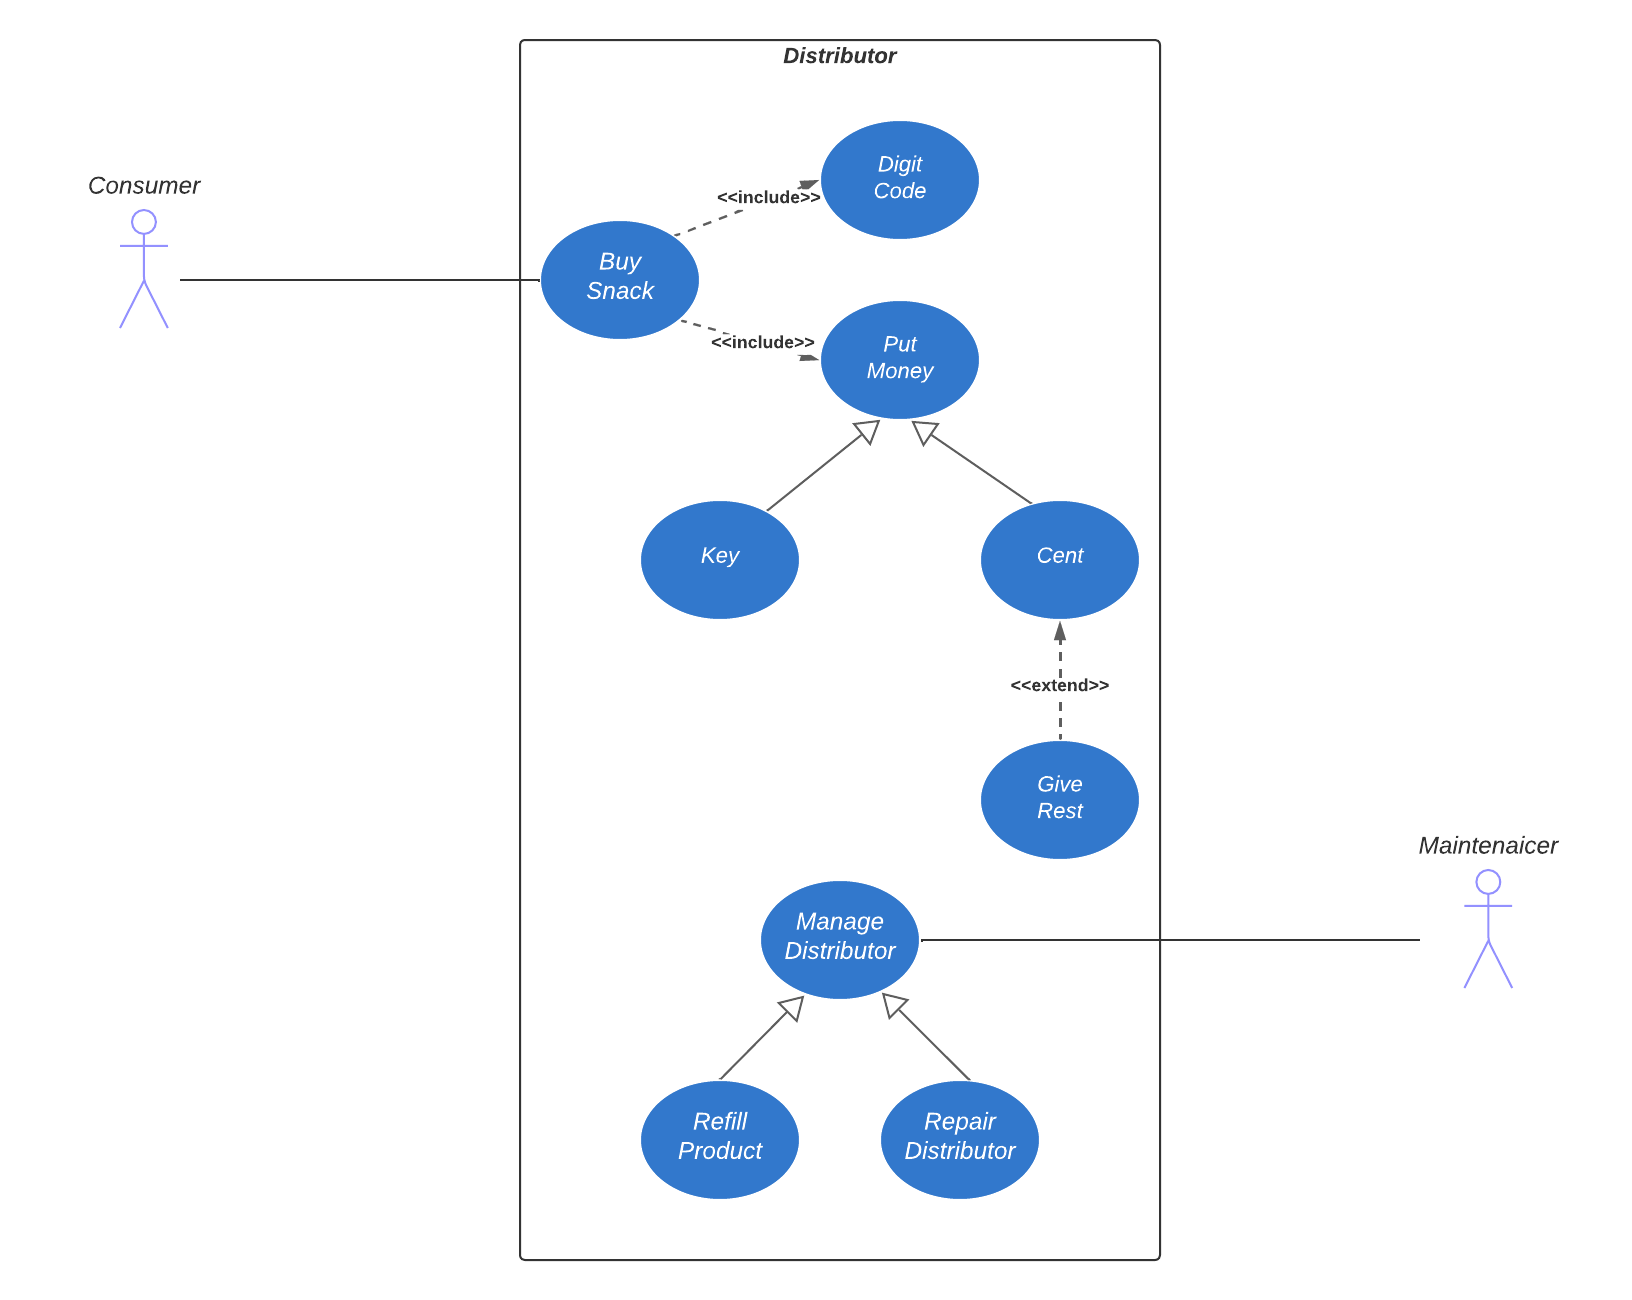
\includegraphics[width=0.9\textwidth]{foto 1.png}
\end{center}
\subsubsection*{Considerazioni}
\large
In questa sezione sono considerate tutte le osservazioni da parte del professore Rossi, il quale esprime la propria visione rispetto
alle soluzioni proposte (\textit{dato che all'esame attua il proprio modo di essere è bene considerare tale sezione, in maniera tale che alla prova d'esame sia meno afflittivo possibile}).\vspace*{14pt}\\
\textit{Considerazioni diagramma}\\
E' bene omettere il caso d'uso \textit{GIVE CHANGE}, poichè non implica un passaggio che non possa essere percepito, tuttavia non rappresenta un errore ma appesantisce la rappresentazione a discapito di un'agevole lettura.
Durante la fase di pagamento, come avviene nell'use case \textit{PUT MONEY}, è buona regola indicare tramite l'operatore logico \textit{XOR}, affinchè solo uno dei due casi d'uso successivi, referenziati tramite l'attributo \textit{include}, possa essere valorizzato.
Scelta accettabile tramite \textit{include}, dato che rappresentano \textit{behavior} fondamentali per conseguire nell'obiettivo dell'attore principale, ossia l'\textit{acquisto di snack o bevande}. Infine, mai aggiungere note supplementari, non citate dalla traccia, poichè potrebbero condurre all'errore e rendere meno comprensivo il diagramma, come avviene per la figura del \textit{Maintenaicer}.\vspace{14pt}\\
\textit{Considerazioni generali}\\
Rispetto a tutti i diagrammi proposti sarebbe stato possibile creare un unico caso d'uso, ossia \textit{BUY ITEM}, il quale avrebbe reso banale il diagramma, ma maggiormente complesso il \textit{Happy Path}. Infatti questo rappresenta una duplice modalità di approccio, dove l'implementazione di un diagramma del genere renderebbe maggiormente complicata la descrizione testuale; quindi è bene porre una corretta via di mezzo, che garantisca un corrispettivo livello informativo sia per il diagramma e, conseguentemente, per la descrizione del main sequence.
\end{document}